\chapter{Introduzione}
In questa sezione, vengono illustrati gli aspetti teorici utili a comprendere l'esperimento mostrato nel \cref{ch:esperimento}. In particolare, sarà fatta una panoramica degli algoritmi di \textit{short term scheduling} (evidenziandone i parametri qualitativi), un cenno alla teoria delle code e all'architettura \textit{client-server}.

\section{Definizioni}

\paragraph{Flusso}\cite{shreedhar1996efficient}
Un flusso è un insieme di richieste che necessita di avere la stessa \textit{Quality of Service} QoS.

\paragraph{Coda}\cite{stallingsos}(p. 21-10)
Una coda è una struttura in cui vengono memorizzate le richieste di un flusso in ingresso e da cui viene gestito l'accesso alla risorsa contesa.

\paragraph{Richiesta}
In questo elaborato, per richiesta si intende un'operazione da effettuare su una risorsa condivisa e che quindi necessita di una politica di \textit{scheduling}. In particolare, facendo riferimento al processore come risorsa contesa, spesso, una richiesta viene indicata anche come processo.

\section{Algoritmi di \textit{short term scheduling}}\label{s:scheduling}
Gli algoritmi di \textit{short term scheduling} sono utilizzati per scegliere quale processo (tra quelli pronti) deve essere eseguito dal processore e mirano a migliorare le prestazioni di un sistema. Prima di analizzare gli approcci utilizzati, è importante effettuare una panoramica dei parametri utilizzati per valutare le \textit{performance} di un sistema. In particolare, questi si dividono in:
\begin{itemize}
    \item \textbf{\textit{System oriented}}: valutano l'efficienza di un algoritmo di \textit{scheduling} dal punto di vista del sistema. Sono riassunti in \cref{tab:sys_oriented};
    \item \textbf{\textit{User oriented}}: esprimono le prestazioni dell'algoritmo dal punto di vista dell'utente che utilizza il sistema. Sono riassunti in \cref{tab:user_oriented};
\end{itemize}

In entrambe le classi di parametri presentate, possono essere distinti altri criteri oltre a quelli legati alle \textit{performance} del sistema come, ad esempio, gestione delle risorse, gestione delle priorità, predicibilità, \textit{fairness} etc. \cite{stallingsos}.

\begin{table}[h]
    \centering
    \begin{tabular}{|p{2.5cm}||p{9cm}| }
        \hline
        Parametro & Descrizione \\ [0.5ex] 
         \hline\hline
         \hline
         \textit{Throughput}& Numero di processi completati in un intervallo temporale.\\
         \hline 
         \hline
         \textit{Utilizzazione del processore}& Percentuale del processore utilizzata. In generale, un processore ha una capacità $\rho$ che viene condivisa tra i processi. In particolare, se $n$ è il numero di processi nel sistema, allora $\mu=\frac{n}{p}$ è l'utilizzazione del processore. Inoltre, vale la seguente relazione $\mu \leq 1$ \\
         \hline
    \end{tabular}
    \caption{Parametri \textit{system oriented}.}
    \label{tab:sys_oriented}
\end{table}

\begin{table}
    \centering
    \begin{tabular}{|p{2.5cm}||p{9cm}| }
        \hline
        Parametro & Descrizione \\ [0.5ex] 
         \hline\hline
         \hline
         \textit{Turnaround Time}& Tempo totale che il processo trascorso all'interno del sistema, tenendo conto di quello che spende sia in attesa di risorse che in esecuzione. In seguito viene anche indicato con \textit{residence time}.\\
         \hline 
         \hline
         \textit{Response time}& Tempo trascorso dalla sottomissione del processo alla risposta data all'utente.\\
         \hline
         \hline
         \textit{Deadline}& La \textit{deadline} indica il tempo entro cui il processo deve produrre un risultato.\\
         \hline
    \end{tabular}
    \caption{Parametri \textit{user oriented}.}
    \label{tab:user_oriented}
\end{table}

\subsection{Starvation}

Alcune \textit{policy} di \textit{scheduling} soffrono di \textit{starvation}\cite{stallingsos}: questi algoritmi mirano a privilegiare delle classi di processi facendo si che altre non vengano mai eseguite. Una prima strategia per contenere il fenomeno della \textit{starvation} è quello di introdurre il concetto di prelazione all'interno degli algoritmi in modo tale da evitare che un singolo processo monopolizzi la CPU. Un altro modo per risolvere il problema consiste nell'introduzione di meccanismi a priorità dinamica (\textit{aging}) facendola aumentare al crescere del tempo di permanenza dei processi nel sistema. La presenza di \textit{starvation} può essere controllata lavorando sulla \textit{fairness} di un algoritmo di \textit{scheduling}. In particolare, sopratutto nelle applicazioni di rete, è importante garantire che nessun processo monopolizzi le risorse di sistema. Ad esempio, all'interno di un \textit{router} è necessario che tutte le code di ingresso riescono ad eseguire l'instradamento dei pacchetti senza impattare troppo sulle latenze.

\subsection{Principali algoritmi di scheduling}

Di seguito vengono descritti brevemente alcuni approcci utilizzati per gli algoritmi di \textit{scheduling}; mentre in \cite{stallingsos}(p. 434) sono schematizzati come questi si comportano in relazione ai parametri presentati in \cref{s:scheduling}.

\paragraph{First Come First Served (FCFS)}
L'approccio più semplice è il cosiddetto \textit{First Come First Served}: i processi vengono serviti nell'ordine in cui arrivano. Si tratta del tipo di \textit{policy} più semplice in cui è presente una sola coda. In questo algoritmo, i processi lunghi tendono a monopolizzare la CPU a sfavore dei processi brevi che soffrono di \textit{starvation}.

\paragraph{Round-robin}
L'algoritmo \textit{round-robin} è una versione \textit{preemptive} di \textit{FCFS} in cui il processore viene condiviso tra i processi con la tecnica del \textit{time slicing}. In generale, gli algoritmi \textit{round-robin} consentono di gestire più flussi che si contendono l'accesso a una risorsa (in questo caso il processore), ma soffrono di un problema di \textit{fairness}: pur allocando lo stesso quanto di tempo, i flussi possono avere caratteristiche (\textit{rate}, dimensione dei pacchetti etc.) differenti e pertanto il \textit{throughput} presentato in uscita non è equo. Inoltre, la scelta del quanto di tempo risulta problematica. In generale, un quanto di tempo piccolo consente di migliorare il tempo di risposta dei processi brevi, ma se troppo breve comporta un'esecuzione troppo frammentata e può rendere lo \textit{scheduling} inefficiente contando i costi di \textit{context switch} e complessità computazionale dell'algoritmo.

\paragraph{Shortest Job Next}
Gli algoritmi di \textit{scheduling} di questo tipo eseguono prima i processi brevi. Benché questi siano noti per fornire le prestazioni migliori (alto \textit{throughput} e un buon tempo di risposta), tendono a far soffrire di \textit{starvation} i processi lunghi. Inoltre, nella pratica è molto difficile stimare il tempo di esecuzione di un processo. Per i processi che eseguono più volte, vengono calcolate statisticamente delle metriche dando più importanza alle esecuzioni più recenti.

\subsection{Algoritmo Deficit Round Robin (DRR)}\label{s:drr}
In questo elaborato, viene posta l'attenzione sull'algoritmo DRR in quanto viene utilizzato nell'esperimento descritto in \cref{ch:esperimento}. L'algoritmo fu proposto nel 1995 come una soluzione \textit{fair} e più efficiente (complessità O(1)) del generico \textit{Weighted Fair Queuing} (WFQ)\cite{wiki:drr}. Quest'approccio nasce per equilibrare il numero di \textit{byte} (in particolare si parla di pacchetti) inviati su una coda e di solito viene implementato in contesti di \textit{networking}.\\
In generale, il DRR è una versione \textit{stateful} del \textit{round-robin} e si basa sull'introduzione di variabili di stato\cite{shreedhar1996efficient} che tengono traccia del \textit{throughput} di ciascun flusso ingresso e sul \textit{mapping} di questi in altrettante code a priorità. L'operazione di \textit{mapping} avviene secondo l'algoritmo \textit{Stochastic Fair Queuing} (SFQ) \cite{shreedhar1996efficient} che prevede il calcolo di un \textit{hash} per l'assegnazione di un pacchetto ad una coda. In questo elaborato, il DRR viene utilizzato per implementare un algoritmo di \textit{scheduling} a priorità assegnando un peso diverso ai flussi in ingresso, come mostrato in \cref{ch:esperimento}.

\section{Teoria delle code}
All'interno dell'analisi delle prestazioni, la teoria delle code gioca un ruolo fondamentale in quanto fornisce gli strumenti matematici per modellare il carico di lavoro (\textit{workload}) di un servizio e dei parametri statistici per valutarne le \textit{performance} senza perdere di generalità. In particolare, in questa sezione sarà descritto il modello a singola coda con una verticalizzazione sui principali parametri per l'analisi delle prestazioni descritti in \cref{tab:sys_oriented} e \cref{tab:user_oriented}. Prima di descrivere il modello a singola coda, saranno introdotte la notazione di Kendall e la distribuzione di Poisson, evidenziando la loro utilità all'interno della teoria delle code.\newline
Come premessa, nell'ambito della teoria delle code, è improprio parlare di istanti di tempo e intervalli temporali precisi, ma bisogna far riferimento a distribuzioni di probabilità descritte attraverso la loro caratterizzazione sintetica come valore medio, deviazione standard e varianza.

\subsection{Notazione di Kendall}
Nella teoria delle code, i modelli vengono espressi usando la notazione di Kendall\cite{bolch2006queueing} che ne sintetizza i parametri di funzionamento utilizzando la struttura $A/B/m/K\;-\;policy\;di\;scheduling$ in cui con $A$ si indica la distribuzione dei tempi di inter-arrivo delle richieste, $B$ la distribuzione dei tempi di servizio, $m$ il numero dei server a disposizione e $K$ la dimensione del \textit{buffer} per memorizzare le richieste\footnote{Nei modelli con dimensione finita, quando il \textit{buffer} è pieno ogni richiesta viene scartata e risulta persa per sempre.}\cite{bolch2006queueing}(pp. 210-211). In generale, quando il parametro $K$ non viene specificato il sistema si assume con memoria infinita. Inoltre, insieme alla struttura del sistema viene indicata anche la \textit{policy} di \textit{scheduling} utilizzata per servire le richieste. Ad esempio, secondo la notazione di Kendall, la dicitura $M/G/1\;-\;FCFS\;preemptive\;resume\;(PR)$ indica un sistema il cui tempo di inter-arrivo delle richieste varia secondo una distribuzione esponenziale ($M$), il tempo di servizio delle richieste ($G$) è una distribuzione arbitraria, un solo server ($1$), algoritmo di \textit{scheduling} \textit{FCFS preemptive} e \textit{buffer} infinito.

\subsection{Distribuzione di Poisson}\label{poisson}
La distribuzione di Poisson è importante nella teoria delle code poiché esprime un modello secondo cui il tempo di arrivo di una richiesta è indipendente da quello delle altre.

Formalmente, la distribuzione di Poisson è una variabile aleatoria discreta e può essere espressa\cite{stallingsos}(p. 20-9) con:

\begin{equation}
    Pr\;[k\;eventi\;arrivano\;nell'\;intervallo\;T] = \frac{(\lambda T)^k}{k!} e^{-\lambda T}
    \label{eq:poisson1}
\end{equation}

Nella teoria delle code, i processi che arrivano con distribuzione di Poisson vengono indicati come casuali, poiché, come mostrato nella \cref{eq:poisson1}, non è possibile predire, conoscendo il tempo di arrivo di un'occorrenza di un evento, quando arriverà il prossimo. Partendo dalla \cref{eq:poisson1}, è possibile calcolare la media di questa variabile ottenendo:

\begin{equation}
    E\;[eventi\;che\;arrivano\;nell'\;intervallo\; T] = \lambda T
    \label{eq:poisson2}
\end{equation}

In \cref{fig:poisson}, è mostrato l'andamento della distribuzione di \textit{Poisson} al variare di $\lambda$.


\begin{figure}[ht]
  \centering
  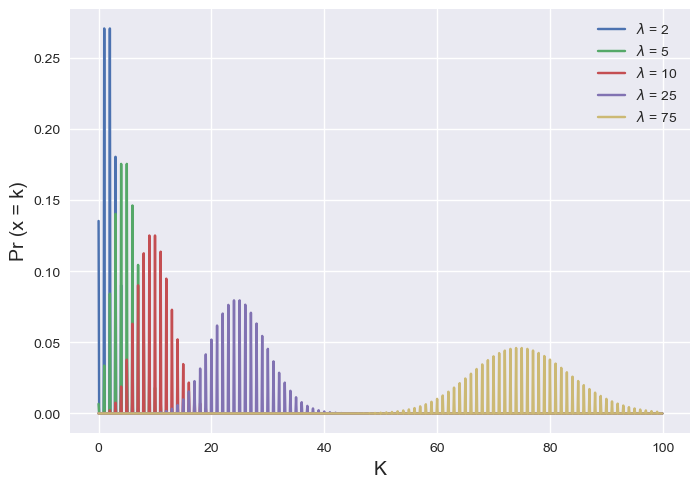
\includegraphics[width=\textwidth]{img/math/poisson.png}
  \caption{Distribuzione cumulativa della variabile di Poisson al variare di $\lambda$ con $T=1$.}
  \label{fig:poisson}
\end{figure}

\begin{figure}[ht]
  \centering
  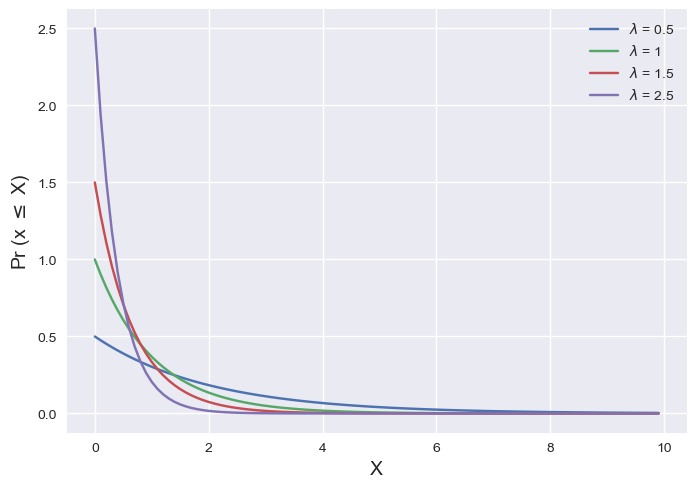
\includegraphics[width=\textwidth]{img/math/exponential.png}
  \caption{Distribuzione di probabilità della variabile esponenziale al variare di $\lambda$.}
  \label{fig:exponential}
\end{figure}

Una importante proprietà della distribuzione di Poisson è la sua relazione con la distribuzione esponenziale (\cref{fig:poisson}). Infatti, così come la distribuzione binomiale esprime il numero di successi in $n$ prove indipendenti (prove di Bernoulli\cite{gelliprobabilita}) e quella geometrica l'intervallo di tempo tra due successi consecutivi, così la distribuzione di Poisson fornisce una stima del numero di eventi in un intervallo finito $T$ e l'esponenziale mette in risalto la distanza temporale tra due eventi consecutivi. Formalmente, questa relazione è messa in evidenza dal tempo di inter-arrivo ($T_a$) tra due eventi che segue un andamento esponenziale\footnote{Si noti che la relazione sussiste tra una variabile aleatoria continua e una discreta}:
\begin{equation}
    Pr\;[T_a < t ] = 1 - e^{-\lambda t}
    \label{eq:cdf}
\end{equation}

Questa proprietà è messa in risalto dal fatto che il tempo di inter-arrivo degli eventi della distribuzione esponenziale coincide con:

\begin{equation}
    E\;[T_a] = \frac{1}{\lambda}
    \label{eq:interarrival}
\end{equation}

mentre il numero medio di eventi al secondo della distribuzione di Poisson è dato dal \textit{rate}:

\begin{equation}
    Mean = \lambda
    \label{eq:rate}
\end{equation}

Pertanto, la relazione che lega la distribuzione di Poisson alla variabile aleatoria esponenziale è la reciprocità tra \textit{rate} di Poisson e tempo di inter-arrivo esponenziale:
\begin{equation}
    E\;[T_a] = \frac{1}{mean}=\frac{1}{\lambda}.
\end{equation}


\subsection{Modello a singola coda}\label{s:mm1}
In base a quanto illustrato in \cref{poisson}, in questo elaborato i tempi di inter-arrivo e di servizio sono assunti casuali e, quindi esponenziali. Secondo la notazione di Kendall, $A=B=M$; mentre utilizzando un solo server $m=1$. Pertanto, il modello utilizzato si chiama a singola coda e viene indicato con $M/M/1$ (schematizzato in \cref{s:mm1}). Di seguito sono mostrati i parametri di \textit{performance} più importanti per i sistemi a singola coda\cite{bolch2006queueing}.

\begin{figure}
  \centering
  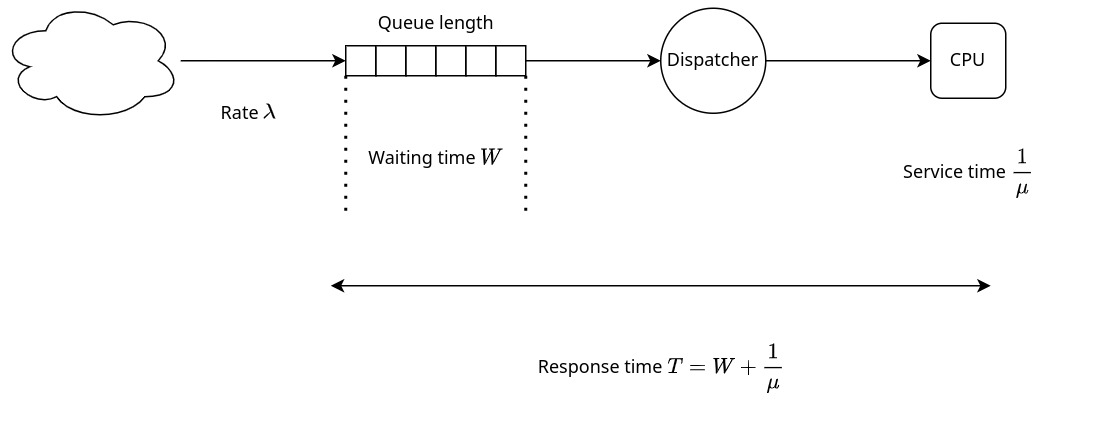
\includegraphics[width=\textwidth]{img/arch/tesi-Pagina-4.jpg}
  \caption{Schema modello a singola coda $M/M/1$.}
  \label{fig:mm1}
\end{figure}


\paragraph{Utilizzazione del processore $\rho$}\cite{bolch2006queueing}
Nei modelli a singola coda, la porzione di tempo per cui il processore risulta occupato dipende dal tempo di inter-arrivo ($\lambda$) dei processi e dal tempo di servizio ($\mu$). In particolare:
\begin{equation}
    \rho = \frac{\lambda}{\mu}
\end{equation}

Inoltre, la condizione per la stabilità per un sistema è $\rho < 1$.

\paragraph{Throughput}

Come accennato in \cref{tab:server_spec}, il \textit{throughput} è una misura per indicare quante richieste vengono servite in un intervallo di tempo. Nei sistemi a singola coda con memoria infinita, il \textit{throghput} è pari a $\lambda$ in quanto nessun processo viene rifiutato. In realtà, questo valore viene saturato in base alla dimensione $K$ del buffer delle richieste e vale la relazione $K \leq n$, con $n$ numero di richieste che arrivano al sistema.

\paragraph{Tempo di attesa}
Il tempo di attesa è il tempo che una richiesta spende nel sistema quando non usufruisce della CPU. In particolare, detto $\overline{T}$ il tempo di risposta (o tempo di residenza), l'intervallo che il processo spende nel sistema, allora si può definire il tempo di attesa $\overline{W}$ come:

\begin{equation}
    \overline{W} = \overline{T} - \frac{1}{\mu}
\end{equation}

\paragraph{Numero di processi nel sistema $K$}
Il numero di processi in un sistema è uno dei più importanti parametri dei sistemi a singola coda e dipende dalla probabilità di avere processi nel sistema $\pi_k$. In particolare, il numero di processi nel sistema può essere espresso come\cite{bolch2006queueing}:
\begin{equation}
    \overline{K} = \sum_{k=1}^{\infty}k\pi_k
\end{equation}

Inoltre, grazie alla legge di Little\cite{wiki:littlelaw}, $\overline{K}$ può essere calcolato come:
\begin{equation}
    \overline{K} =\lambda\overline{T}
\end{equation}
dove con $\overline{T}$ è stato indicato il tempo di risposta medio di una richiesta. Analogamente, la dimensione media della coda $\overline{O}$ può essere espressa, secondo la legge di Little, in funzione del tempo medio di attesa $\overline{W}$:

\begin{equation}
    \overline{O} =\lambda\overline{W}
\end{equation}

\subsection{Stabilità}
Una delle proprietà fondamentali del modello a singola coda è la stabilità. Infatti, con i risultati della teoria di Markov\cite{bolch2006queueing}(capp. 2-3), è possibile studiare il comportamento del modello una volta raggiunta una condizione di regime. Il primo valore che si ricava dagli studi di Markov è la probabilità che la coda sia vuota $\pi_o$:

\begin{equation}
    \pi_0 = \frac{1}{1+\sum\limits_{k=1}^\infty \prod\limits_{i=0}^{k-1} \frac{\lambda}{\mu}} = 1 - \frac{\lambda}{\mu} = 1 - \rho
    \label{equation:pi0}
\end{equation}
Inoltre, si dimostra che la probabilità $\pi_k$ di avere $K$ processi all'interno della coda dipende dall'utilizzazione del processore, come mostrato di seguito:

\begin{equation}
    \pi_k = \pi_0 \left(\frac{\lambda}{\mu}\right)^k
    \label{equation:pik}
\end{equation}

Quindi, ricordando che $\frac{\lambda}{\mu} = \rho$ e sostituendo la \ref{equation:pi0} nella \ref{equation:pik}, si ottiene che:

\begin{equation}
    \pi_k = (1 - \rho)\rho^k
\end{equation}

L'ultima relazione indica che la probabilità del numero di processi all'interno del sistema varia secondo una distribuzione geometrica (il cui andamento è mostrato \cref{fig:geometric}). Pertanto, il numero medio dei processi nel sistema risulta:
\begin{equation}
    \overline{K} = \frac{\rho}{1-\rho}
\end{equation}

\begin{figure}[ht]
  \centering
  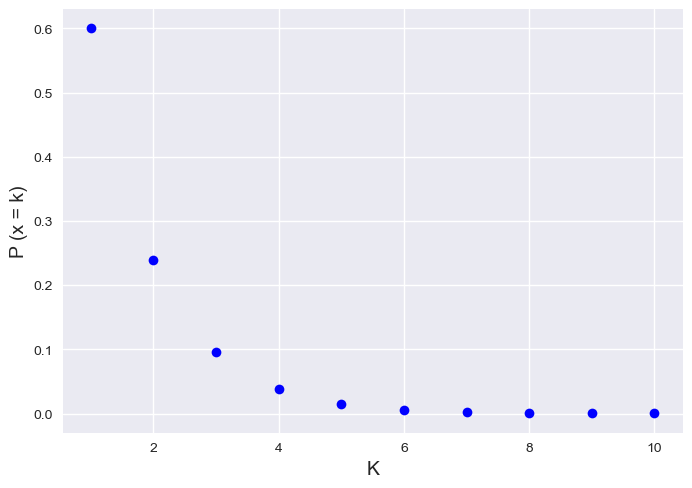
\includegraphics[width=\textwidth]{img/math/geometric.png}
  \caption{Andamento distribuzione geometrica con $\rho=0.6$}
  \label{fig:geometric}
\end{figure}

\section{Architettura client-server}
Nell'esperimento presentato in \cref{ch:esperimento}, è utilizzato il modello architetturale \textit{client-server} in cui sono distinti due tipi di processi:

\begin{itemize}
    \item \textbf{\textit{Server}}: processi che mettono a disposizione dei servizi;
    \item \textbf{\textit{Client}}: processi che fruiscono dei servizi offerti dal server;
\end{itemize}
In questa architettura, il processo \textit{server} resta in attesa di richieste che possono arrivare in maniera concorrente da uno o più \textit{client}. Infatti, sono sempre i \textit{client} ad iniziare la comunicazione con il server, e in generale, una comunicazione può essere composta da un'interazione complessa come nel caso di connessioni TCP.
